\subsection{Confidence calibration changes counting conclusions}
\label{sec:calibration}

A detector produces a ranked list of boxes with confidence scores; a count is
obtained by keeping every box above a threshold. The threshold therefore
controls how many fruit are reported, even when the ranking of the boxes stays
the same. This subsection examines how a fixed threshold can reverse a
comparison between two training recipes.

Three YOLO11n recipes were trained on Laboro under the protocol of
Table~\ref{tab:cross} and scored on tomatOD: the default recipe; the same
recipe with the HSV colour jitter switched off (\texttt{no\_colour}); and the
default with CutMix and mixup added (\texttt{occlusion\_aug}). At the usual
threshold of 0.25 the cross-domain counting MAE is 3.29 for the default, 3.01
for \texttt{occlusion\_aug}, and 1.50 for \texttt{no\_colour}. At this fixed
threshold, removing the colour jitter appears to halve the counting error on
an unfamiliar dataset.

The results at 0.25 are chiefly explained by the number of boxes that each
model returns. The default model predicts 1.92 times as many fruit as tomatOD
contains, while the \texttt{no\_colour} model predicts 0.93 times as many. Their
stage accuracy on matched fruit differs by less than 0.006. The models therefore
assign similar stages to matched fruit but place their confidence scores
differently relative to the threshold. This difference is a property of
calibration.

\begin{table}[t]
\centering
\caption{Counting on tomatOD by three Laboro-trained YOLO11n recipes, at the
fixed threshold of 0.25 and at each model's best threshold from a sweep over
0.05--0.90. Ratio: predicted over annotated fruit at the best threshold.}
\label{tab:calibration}
\setlength{\tabcolsep}{4pt}
\begin{tabular}{lccccc}
\toprule
& MAE & \multicolumn{4}{c}{At the best threshold}\\
\cmidrule(lr){3-6}
Recipe & @0.25 & MAE & conf. & recall & ratio \\
\midrule
default              & 3.29 & 1.34 & 0.70 & 0.799 & 0.88 \\
\texttt{no\_colour}   & 1.50 & 1.50 & 0.25 & 0.746 & 0.93 \\
\texttt{occlusion\_aug} & 3.01 & 1.32 & 0.70 & 0.776 & 0.85 \\
\bottomrule
\end{tabular}
\end{table}

Table~\ref{tab:calibration} sweeps the threshold. The default model reaches
1.34 at confidence 0.70 and keeps a recall of 0.799; the \texttt{no\_colour}
model is already at its best at 0.25, with 1.50 and a recall of 0.746. Once
each model uses its best operating point, meaning the selected confidence
threshold and the resulting recall, the ordering reverses. The colour-jittered
model has lower counting error on the unfamiliar dataset and retains more
recall. The \texttt{no\_colour} model appeared better because its calibration
was closer to the fixed threshold. The mAP result does not change
because mAP averages over every threshold.

Threshold selection also affects the transfer results in
Section~\ref{sec:annotation}. The Laboro model's counting MAE on tomatOD falls
from 3.29 at 0.25 to 1.34 at its best threshold. Threshold selection therefore
accounts for more than half of the apparent transfer penalty in
Table~\ref{tab:cross}; the change of dataset does not account for all of it. On
Laboro, the sweep retains a smaller advantage for \texttt{no\_colour} (0.93
against 1.03). This agrees with its 0.008 higher mAP50--95, but the comparison
uses a single seed and is not treated as a finding.

\begin{figure*}[t]
  \centering
  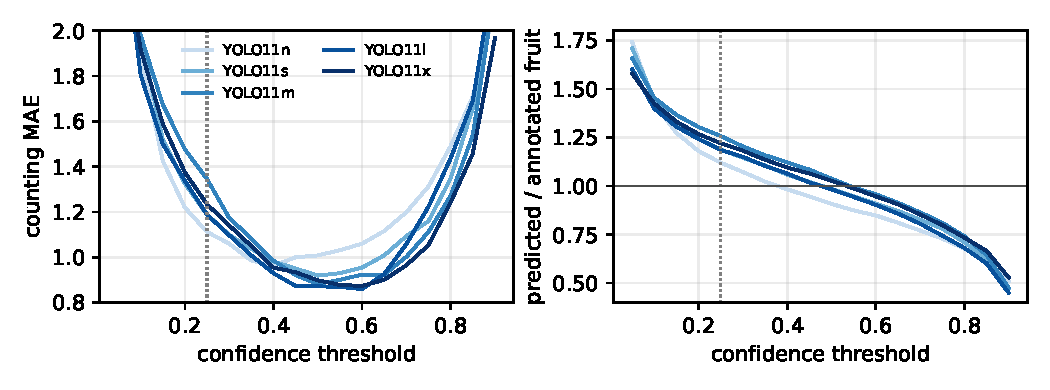
\includegraphics[width=0.85\textwidth]{calibration_curve.pdf}
  \caption{Counting MAE (left) and the ratio of predicted to annotated fruit
  (right) against the confidence threshold, for the five YOLO11 sizes on the
  Laboro validation split. The dotted line marks the default threshold of
  0.25. Every size over-counts at 0.25, and the threshold at which the ratio
  crosses 1.0 differs between sizes.}
  \label{fig:calibration-curve}
\end{figure*}

Figure~\ref{fig:calibration-curve} shows the same mechanism in-domain, across
the model-size ladder of Section~\ref{sec:ladder}. At 0.25 every size predicts
between 1.12 and 1.26 times as many fruit as are annotated, and its counting
MAE is 0.15--0.46 above its own minimum. The error curves are flat between
roughly 0.4 and 0.65 and rise steeply on either side. Their minima lie at
thresholds from 0.40 (YOLO11n) to 0.60 (YOLO11l and x). A single fixed threshold
therefore favours some sizes over others (Table~\ref{tab:ladder-thresh}).

CutMix and mixup were added to test whether pasting image regions over the
fruit during training makes the detector more robust to the occlusion of
Section~\ref{sec:occlusion-results}. The results do not show greater robustness.
Under the background strip, the augmented model reaches recall 0.671 against
the default's 0.694 at 30\% hidden, and 0.283 against 0.312 at 50\%. Its small
advantage in tuned counting on tomatOD (1.32 against 1.34) is well within
single-seed noise. Rectangular occlusion during training therefore provides no
evidence of robustness to either the test intervention or natural leaves.
